There are  many reasons why the LT3741 was chosen to regulate the output voltage
of this device. The most important reasons are listed here.
\begin{itemize}
    \item \textbf{Re-inventing the wheel.}
        Switch-mode regulators aren't new technology. They've been studied and perfected
        over decades by many engineers. For  this  reason  we decided against building a
        regulator  descretely  and  instead  opted  to  use  an  existing  regulator  if
        available.
    \item \textbf{Voltage and current requirements.}
        The device is specified to  output  voltage  levels  between  \SI{0}{\volt}  and
        \SI{24}{\volt} and current levels between \SI{0}{\ampere} and \SI{3.5}{\ampere}.
        Further,  the  ripple voltage is specified to be $\le\SI{300}{\milli\volt}$  and
        the ripple current  is  specified to be $\le\SI{100}{\milli\ampere}$. The LT3741
        fulfills all of these requirements.
    \item \textbf{The importance of power absorption.}
        Most switch-mode  regulators  are  only  able  to  \emph{supply}  power, but are
        incapable  of  \emph{absorbing} power. Because our device may  be  connected  in
        series (or parallel) with other power  supplies,  it  must  have  the ability to
        absorb  power  to  (which is the case if, say, it were connected  to  a  voltage
        source   outputting   a   higher  voltage  level  than  our  own).  A  so-called
        \emph{synchronous  converter} possesses this property and the LT3741 is  one  of
        them.
    \item \textbf{Control inputs.}
        The LT3741 was chosen  because  it has dedicated input control pins for directly
        changing  the  regulated  output  current.  This makes the design a lot simpler,
        because no complicated additional circuitry is required.
\end{itemize}

\begin{figure}[th!]
    \center
    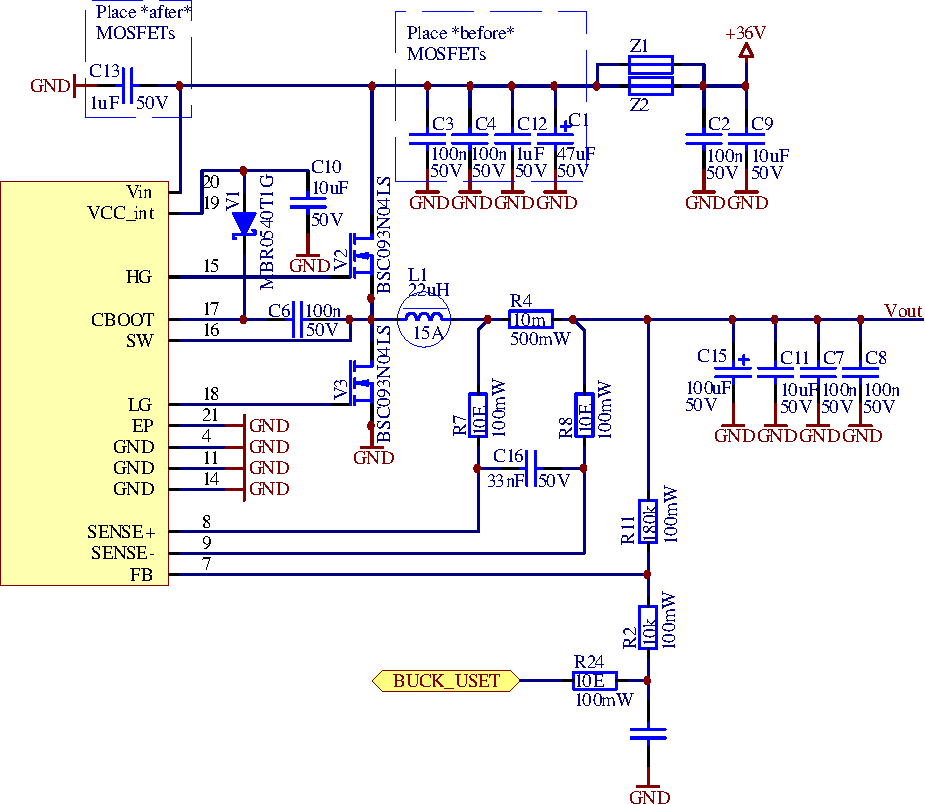
\includegraphics[width=.75\textwidth]{images/circuit/buck.pdf}
    \caption{Herzst\"uck des Projektes: Aufbau des LT3741 CVCC Synchronwandler}
    \label{fig:circuit:buck}
\end{figure}

With the LT3741 selected, the selection of  components  required  to control the
LT3741 are discussed next.

% **************************************************************************** %
\subsubsection{Bypass Capacitors}
% **************************************************************************** %

The LT3741 is powered by the \SI{28}{\volt}  rail, which can be seen in Figure
\ref{fig:circuit:buck} in the  top right. The switching of  the MOSFETs causes
the LT13741  to consume high amounts  of power in short  bursts. This leads to
the LT3741  feeding high  frequency disturbance  back into  the \SI{28}{\volt}
rail, which  could lead  to disturbances  in the  rest of  the circuit  if not
handled correctly.  As a countermeasure,  a multitude of different ceramic and
electrolytic bypass  capacitors in parallel  are used.  Additionally,  we used
ferrite beads, placed  in series with the supply to  absorb any high frequency
feedback.


% **************************************************************************** %
\subsubsection{Switching Frequency}
% **************************************************************************** %

There is a trade-off when  selecting the switching frequency $f_S$. The higher
$f_S$,  the  lower the  output  ripple  voltage  will be. However,  the  power
consumption will also  increase due to switching losses.   Generally, $f_S$ is
to be maximised to reduce ripple.

Because so  much depends  on $f_S$,  it is more  convenient to  determine this
value empirically through simulations. The  most sutiable value was determined
to be $f_S \approx\SI{800}{\kilo\hertz}$. In the remaining calculations, $f_S$
is assumed to be \SI{1}{\mega\hertz} to allow for some leeway.

A specific  resistor on one  of the LT3741's inputs  is used to  configure the
switching frequency $f_S$.


% **************************************************************************** %
\subsubsection{Inductor Selection}
% **************************************************************************** %

The size of the inductor $L_1$, as illustrated in figure \ref{fig:circuit:buck},
was calculated using formula \ref{eq:circuit:buck:inductor}
\begin{equation}
    L_1 = \left( \frac{U_{in} \cdot U_{out} - U_{out}^2}{0.3 \cdot f_S \cdot I_O \cdot U_{in}} \right) = \SI{6}{\micro\henry}
    \label{eq:circuit:buck:inductor}
\end{equation}
where $U_{in}$ is the  input  voltage  \SI{28}{\volt},  $U_{out}$  is the output
voltage at peak power (which exists at $U_{out} = \SI{14}{\volt}$), $f_S$ is the
switching frequency \SI{1}{\mega\hertz} and $I_o$ is the maximum output current,
assumed   to   be   $I_o  =  \SI{5}{\ampere}$  for   some   additional   leeway.

We ended up selecting a  larger  inductor  of  $L_1  = \SI{22}{\micro\henry}$ to
further decrease ripple current.

In addition to the value of  the  inductor, the maximum current rating, DCR, and
saturation  current are also important factors to consider. The maximum  current
of the inductor is calculated using formula 
\ref{eq:circuit:buck:inductor_peak}
\begin{equation}
    I_{L_{1_{peak}}} = I_O + \left( \frac{U_{in} \cdot U_{out} - U_{out}^2}{2 \cdot f_S \cdot L_1 \cdot U_{in}} \right) = \SI{5.2}{\ampere}
    \label{eq:circuit:buck:inductor_peak}
\end{equation}
Where $L$  is  the  value  of  the selected inductor, \SI{22}{\micro\henry}. The
saturation  current  of the inductor was sized factor $1.2$ higher than the peak
current.
\begin{equation}
    I_{L_{1_{saturation}}} = 1.2 \cdot I_{L_{1_{peak}}}
    \label{eq:circuit:buck:inductor_saturation}
\end{equation}

A  list  of  candidates  matching  the  above  parameters  are  listed in  table
\ref{tab:circuit:buck:inductor}.

\begin{table}[th!]
    \begin{center}
        \caption{}
        \label{tab:circuit:buck:inductor}
        \begin{tabular}{lcccc}
            \toprule
            Digikey         & Price (CHF) & Inductance (\SI{}{\micro\henry}) & DCR (\SI{}{\ohm}) & Ohmic Loss (\SI{}{\watt}) \\
            \midrule
            \rowcolor{lightgray}
            732-4237-1-ND   & 8.03        & 22                               & 0.007             & 0.175  \\
            732-2179-1-ND   & 6.4         & 47                               & 0.0335            & 0.8375 \\
            732-2177-1-ND   & 6.4         & 22                               & 0.0146            & 0.365  \\
            \bottomrule
        \end{tabular}
    \end{center}
\end{table}

It  is  clear that the one with the lowest DCR will be the most optimal. The one
highlighted in grey is the one we chose.



% **************************************************************************** %
\subsubsection{MOSFET selection}
% **************************************************************************** %

Die  Bauteile  $V_1$  und  $C_6$  bilden  zusammen  mit  dem  MOSFET  $V_2$  ein
High-Side-Schalter. Im Gegensatz zu einem nicht-synchronen Schaltregler befindet
sich  an  der Stelle wo normalerweise eine Freilaufdiode sein sollte ein zweiter
MOSFET $V_3$. Dieser erm\"oglicht  eine  Spannungsregelung in der gegengesetzten
Richtung -- sprich, sie erm\"oglicht eine Leistungsaufnahme, was, wie oben schon
erw\"ant wurde, kritisch ist.

Bei  der  Auswahl von passenden MOSFETs sind die  Parameter  $Q_G$  (Total  Gate
Charge),  $R_{DS_{(on)}}$  (On-Resistance),  $Q_{GD}$  (Gate to  Drain  Charge),
$Q_{GS}$ (Gate to Source  Charge),  $R_G$  (Gate Resistance), sowie $U_{GS}$ und
$U_{DS}$, $I_{D_{max}}$ und $U_{GS_{THR}}$ kritische Parameter.

Der  maximale  Drain-Strom  kann mit der Formel  \ref{eq:circuit:buck:mosfet_id}
berechnet werden

\begin{equation}
    I_{D_{max}} = I_O + \left( \frac{U_{in} \cdot U_{out} - U_{out}^2}{2 \cdot f_S \cdot L \cdot U_{in}} \right) = \SI{5.2}{\ampere}
    \label{eq:circuit:buck:mosfet_id}
\end{equation}

wobei $I_O$ der maximale Ausgangsstrom  von  \SI{5}{\ampere}  ist,  $U_{in}$ die
Eingangsspannung von  \SI{36}{\volt}  ist,  $U_{out}$  die  Ausgangsspannung bei
gr\"osster  Leistung  ist   (\SI{18}{\volt}),   $f_S$   die  Schaltfrequenz  von
\SI{1}{\mega\hertz}  ist  und  $L$  die  Spule  von  \SI{22}{\micro\henry}  ist.

$U_{DS}$   wurde   h\"oher  gew\"ahlt  als  die  Eingangsspannung:   $U_{DS}   >
\SI{36}{\volt}$.

Der LT3741 liefert als maximale Gate-Steuer-Spannung $U_{GS}$  \SI{5}{\volt}. Da
der LT3741 w\"ahrend dem Aufstartvorgang Steuersignale knapp unter \SI{3}{\volt}
liefert,   muss   die   Gate-Threshold-Spannung   $U_{GS_{THR}}$   kleiner   als
\SI{2}{\volt} gew\"ahlt werden. $U_{GS_{min}}$ muss gr\"osser  als \SI{5}{\volt}
sein.

Leistungsverluste der MOSFETs sind einerseits verbunden mit ohmsche  Verluste --
abh\"angig  von  $R_{DS_{(on)}}$  --  sowie   verbunden  mit  Schaltverluste  --
abh\"angig von $Q_{GS}$ und $Q_{GD}$.

Der    Leistungsverlust    im    High-Side   MOSFET   kann   mit   der    Formel
\ref{eq:circuit:buck:mosfet_ploss} approximiert werden

\begin{multline}
    P_{LOSS} = (\textrm{ohmic loss}) + (\textrm{transission loss}) \\
             \approx \left( I_O^2 \cdot R_{DS_{(on)}} \cdot \rho_T \right)
                    + \left( \frac{U_{in} \cdot I_O}{\SI{5}{\volt}} \cdot \left(Q_{GD} + Q_{GS} \right) \cdot \left( 2 \cdot R_G + R_{PU} + R_{PD} \right) \cdot f_S \right) \\
    \label{eq:circuit:buck:mosfet_ploss}
\end{multline}

wobei $\rho_T$ ein temperaturabh\"angiger Parameter vom Einschaltwiderstand ist.
Bei \SI{70}{\celsius} betr\"agt $\rho_T \approx 1.3$. $R_{PD}$ und $R_{PU}$ sind
die  Ausgangsimpedanzen  vom  LT3741  und  betragen  \SI{1.3}{\ohm}   respektive
\SI{2.4}{\ohm}.

Der  Low-Side MOSFET sollte einen m\"oglichst kleinen $R_{DS_{(on)}}$ haben  und
ein    Total-Gate-Charge    $Q_C    \leq    \SI{30}{\nano\coulomb}$    besitzen.

Ein  weiterer Verlust sind die Schaltverl\"uste der internen  MOSFET-Treiber  im
LT3741. Die Total Gate Charge $Q_C$ muss  w\"ahrend  jedem  Zyklus  geladen  und
wieder   entladen   werden.   Diese   Verl\"uste   k\"onnen   mit   der   Formel
\ref{eq:circuit:buck:switching_loss} berechnet werden,

\begin{equation}
    P_{LOSS\_LDO} \approx \left( (U_{in} - \SI{5}{\volt} \right) \cdot \left( Q_{GLG} + Q_{GHG} \right) \cdot f_S
    \label{eq:circuit:buck:switching_loss}
\end{equation}

wobei $G_{GLG}$ die  Low-Side  Gate-Charge $G_C$ ist und $G_{GHG}$ die High-Side
Gate-Charge ist.

In  der  Tabelle  \ref{tab:circuit:buck:mosfet}  sind  verschiedene MOSFET-typen
aufgelistet, die in den oben genannten Parametern passen. Dabei wurde $P_{LOSS}$
und $P_{LOSS\_LDO}$ f\"ur jeden Kandidaten berechnet.

\begin{table}[th!]
    \begin{center}
        \caption{}
        \label{tab:circuit:buck:mosfet}
        \begin{tabular}{cccccccccc}
            \toprule
            $R_{DS_{(on)}}$ & $Q_{GD}$ & $Q_{GS}$ & $R_G$ & $U_{GS_{THR}}$ & Ohmic Loss & Transision Loss & Total Loss & Drive Loss \\
            \midrule
            0.0032          & 4        & 2.5      & 0.4   & 2.5            & 0.104      & 1.0296          & 1.1336     & 0.806 \\
            0.0039          & 7        & 9        & 2.4   & 3.3            & 0.12675    & 4.8384          & 4.96515    & 1.984 \\
            0.0042          & 7        & 9        & 2.4   & 3.3            & 0.1365     & 4.8384          & 4.9749     & 1.984 \\
            0.008           & 2        & 4.5      & 3     & 2              & 0.26       & 2.2464          & 2.5064     & 0.558 \\
            0.0067          & 5.3      & 3.9      & 1.5   & 1              & 0.21775    & 2.18592         & 2.40367    & 0.7998 \\
            \rowcolor{lightgray}
            0.0093          & 2        & 4.9      & 1     & 2              & 0.30225    & 1.39104         & 1.69329    & 1.488 \\
            0.019           & 8        & 4        & 1.3   & 2              & 0.6175     & 2.6784          & 3.2959     & 1.798 \\
            0.0095          & 7.5      & 6        & 1     & 3              & 0.30875    & 2.7216          & 3.03035    & 1.736 \\
            \bottomrule
        \end{tabular}
    \end{center}
\end{table}

Vergleicht  man  \emph{Total  Loss}  und  \emph{Drive Loss}, w\"ahre der oberste
MOSFET  geeigneter. Aus Kostengr\"unden und  generell  schlechter  Dokumentation
wurde  aber  der   n\"achst  bessere  MOSFET  gew\"ahlt  --  hier  mit  hellgrau
hervorgehoben.

Es  wird  f\"ur  den  High-Side  MOSFET wie auch f\"ur den Low-Side  MOSFET  der
gleiche Typ verwendet.



% **************************************************************************** %
\subsubsection{Measurement of Output Voltage and Output Current}
% **************************************************************************** %

Der  LT3741  ist  sowohl   Spannungsgesteuert   wie   auch  Stromgesteuert.  Der
Spannungsteiler  $R_{11} \parallel R_2$ (siehe Abbildung  \ref{fig:circuit:buck}
oder    Abbildung    \ref{fig:circuit:buck:uset})   erlaubt   das   Messen   der
Ausgangsspannung  und  ein  Shunt-Widerstand  $R_4$   erm\"oglicht   die  genaue
\"Uberwachung des Stromes durch die Spule  $L_1$.  Der Widerstand $R_4$ wurde so
gew\"ahlt damit der  maximale  Ausgangsstrom  maximal  \SI{5}{\ampere}  betragen
kann.

Strom\"uberwachung   ist  sehr  wichtig  bei  einer  solchen  Aufgabe   wo   die
Ausgangsspannung  sich  konstant  \"andert.  Sie erlaubt  genauer  vorhersebares
Verhalten der Spannungs\"anderung am Ausgang -- \"Uberschiessen der Sollspannung
und  extreme  Stromspitzen  in  der  Spule  k\"onnen  besser  vermieden  werden.

Weiter   kann   ein   Stromgesteuerter   Regler  auch  als   Konstantstromquelle
funktionieren. Diese Eigenschaft  ist  vorallem  dann  von  Bedeutung  wenn  der
Arbeitspunkt  sich  im  ``steilen''  bereich  der   UI-Kennlinie  des  PV-Moduls
befindet.

Die  Feedback-Widerst\"ande   $R_2$   und   $R_{11}$   wurden  nach  der  Formel
\ref{eq:circuit:buck:feedback_resistors}       dimensioniert      damit      die
Ausgangsspannung maximal \SI{23}{\volt} betr\"agt.

\begin{equation}
    U_{out} = \SI{1.21}{\volt} \left( 1 + \frac{R_{11}}{R_2} \right)
    \label{eq:circuit:buck:feedback_resistors}
\end{equation}

Die Ausgangsspannung kann  danach  durch Anheben der Bezugsspannung $BUCK\_USET$
nach der  Formel \ref{eq:circuit:buck:uset} ver\"andert werden. 

\begin{equation}
    U_{out} = (\SI{1.21}{\volt} - BUCK\_USET) \cdot \frac{R_{11} + R_2}{R_2}
    \label{eq:circuit:buck:uset}
\end{equation}

Wobei $BUCK\_USET$ die analoge Spannung vom  ersten  DAC  ist.  In der Abbildung
\ref{fig:circuit:buck:uset} ist die dazugeh\"orige Schaltung.

\begin{figure}[th!]
    \center
    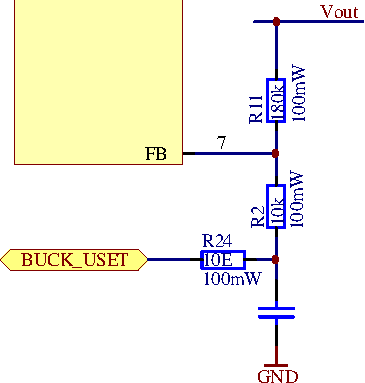
\includegraphics[width=.35\textwidth]{images/circuit/buck-uset.pdf}
    \caption{Einstellung der Ausgangsspannung durch \"Anderung der Bezugsspannung im Feedback-Loop mittels einer analogen Steuerspannung von 0V bis 1.21V}
    \label{fig:circuit:buck:uset}
\end{figure}

Analog zur Ausgangsspannung kann auch der Maximalstrom eingestellt werden. Durch
anlegen einer  analogen  Spannung  zwischen \SI{0}{\volt} und \SI{1.5}{\volt} am
Eingang  CTRL1 des LT3741 kann  direkt  der  maximale  \emph{Durchschnittsstrom}
durch die Spule $L_1$ und  somit  der maximale Ausgangsstrom eingestellt werden.

\begin{figure}[th!]
    \center
    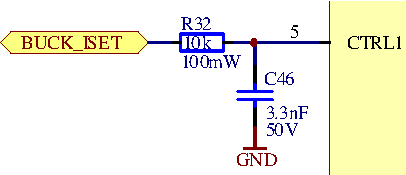
\includegraphics[width=.4\textwidth]{images/circuit/buck-iset.pdf}
    \caption{Einstellung des Maximalstroms mittels einer analogen Steuerspannung von 0V bis 1.5V}
    \label{fig:circuit:buck:iset}
\end{figure}

Die Abbildung \ref{fig:circuit:buck:iset} zeigt  die  dazugeh\"orige  Schaltung.
Der   maximale  durchschnittliche  Ausgangsstrom  $I_o$  wird  mit  der   Formel
\ref{eq:circuit:buck:output_current} berechnet

\begin{equation}
    I_o = \frac{U_{CTRL1}}{30 \cdot R_4}
    \label{eq:circuit:buck:output_current}
\end{equation}

wobei $U_{CTRL1}$ die  analoge  Steuerspannung vom zweiten DAC ist und $R_4$ der
\SI{10}{\milli\ohm}    Shunt-Widerstand    ist,   welcher   in   der   Abbildung
\ref{fig:circuit:buck} zu sehen ist.

Damit der Mikrocontroller angemessene Steuerspannungen  generieren kann, braucht
er die Ausgangsspannung und den Ausgangsstrom zu messen.

Die   Ausgangsspannung   wird   mittels   der   Schaltung   in   der   Abbildung
\ref{fig:circuit:buck:umeas} gemessen. Die Widerst\"ande $R_{12}$  und  $R_{15}$
wurden  so  dimensioniert  damit  die  Spannung  $BUCK\_UMEAS$  im  Bereich  von
\SI{0}{\volt} bis \SI{1.5}{\volt} skaliert ist.

\begin{figure}[th!]
    \center
    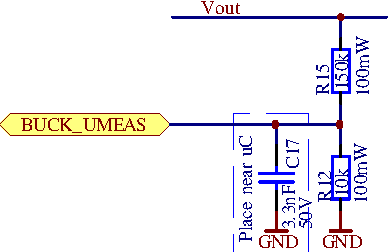
\includegraphics[width=.45\textwidth]{images/circuit/buck-umeas.pdf}
    \caption{Messen der Ausgangsspannung}
    \label{fig:circuit:buck:umeas}
\end{figure}

Der  Ausgangsstrom  wird  mittels  einem  Shunt-Widerstand  $R_5$  differentiell
gemessen.  Die  Schaltung dazu ist in der Abbildung \ref{fig:circuit:buck:imeas}
dargestellt.

\begin{figure}[th!]
    \center
    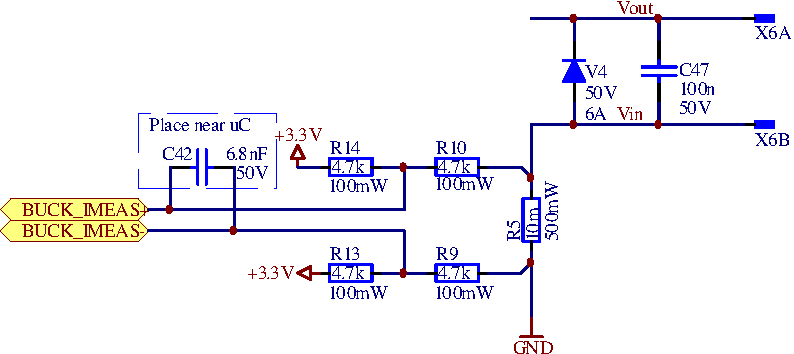
\includegraphics[width=.85\textwidth]{images/circuit/buck-imeas.pdf}
    \caption{Messen des Ausgangsstromes}
    \label{fig:circuit:buck:imeas}
\end{figure}

Es  ist  zu  beachten,  dass  die  Widerst\"ande  $R_{10}$  und  $R_{14}$  einen
Bias-Strom durch den Widerstand $R_5$  verursachen.  Somit  entsteht ein kleiner
Spannungs-Offset.
\begin{equation}
    U_{offset} = \frac{ \SI{3.3}{\volt} \cdot R_5 }{ R_{14} + R_{10} + R_5 }
    \label{eq:circuit:buck:shunt_offset}
\end{equation}

Da   der   ADC   eine   12-bit   Aufl\"osung   mit  einer  Referenzspannung  von
\SI{3.3}{\volt} hat, gilt:
\begin{equation}
    U_{step} = \frac{\SI{3.3}{\volt}}{2^{12}} = \SI{806}{\micro\volt}
    \label{eq:circuit:buck:adc_step}
\end{equation}

Die Widerst\"ande $R_9$, $R_{10}$, $R_{10}$ und  $R_{14}$  sollten  so klein wie
m\"oglich  dimensioniert  werden damit St\"orungen an  den  Leitungen  minimiert
werden  k\"onnen,  aber  sollten immer noch gross genug sein, damit  $U_{offset}
\leq  U_{step}$.  Zu  gross  d\"urfen  sie  auch  nicht  sein,  weil  sonst  die
Holding-Time  des   ADCs   nicht   mehr   erf\"ullt   ist  (was  bei  ca.  $\geq
\SI{5}{\kilo\ohm}$      der      Fall     ist).     Aus     den      Gleichungen
\ref{eq:circuit:buck:shunt_offset} und \ref{eq:circuit:buck:adc_step} kann jetzt
nach den 4 Widerst\"anden aufgel\"ost werden. Es gilt:
\begin{align*}
                          U_{step} &\geq U_{offset} \\
    \frac{\SI{3.3}{\volt}}{2^{12}} &\geq \SI{3.3}{\volt} \cdot \frac{R_5}{R_x + R_5} \\
                  \frac{1}{2^{12}} &\geq \frac{R_5}{R_x + R_5} \\
                               R_x &\geq \left( 2^{12} - 1 \right) \cdot R_5 \\
\end{align*}

wobei  $\frac{R_x}{2}  =  R_{9}  =  R_{10} = R_{13} = R_{14}$. Berechnet  ergibt
$\frac{R_x}{2} \approx \SI{22}{\ohm}$.

Eine weitere Einschr\"ankung, vorallem bei  kleinen  Widerst\"anden,  ist,  dass
nicht  unn\"otig  viel  Leistung  verbraten  werden sollte. Deshalb  werden  die
Widerst\"ande ein wenig h\"oher mit \SI{270}{\ohm} dimensioniert. In diesem Fall
ist der Leistungsverlust aller 4 Widerst\"ande:
\begin{equation*}
    P_{loss} \approx \frac{\SI{3.3}{\volt}^2}{2\cdot \SI{270}{\ohm}} \approx \SI{20}{\milli\watt}
\end{equation*}

Die gemessene Spannung  am  Shunt-Widerstand  ist recht klein. Deshalb verwenden
wir  den  im  Mikrocontroller  eingebauten  vorverst\"arker  (PGA),   was   eine
Verst\"arkung von bis  zu Faktor 64 erreichen kann. Das verst\"arkte Signal wird
intern an der eingebauten differentiellen ADC weitergeleitet.



% **************************************************************************** %
\subsubsection{Output}
% **************************************************************************** %

Two  banana  plugs  $X_{6A}$  and  $X_{6B}$  provide  the  connection  to  the
output  voltage,  while  reverse  voltage protection  is  achieved  via  diode
$V_4$.   (Figure \label{fig:circuit:output}).   An external  reference voltage
of  \SI{1.5}{\volt}  is  used to  ensure  that  the  ADCs  and DACs  can  make
accurate  measurements and  can  be used  over their  full  range (see  figure
\ref{fig:circuit:vref}).

\begin{minipage}{.50\textwidth}
    \center
    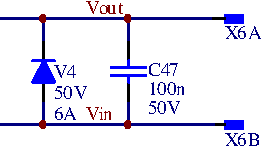
\includegraphics[width=.9\textwidth]{images/circuit/output-connectors.pdf}
    \captionof{figure}{Reverse voltage protection at output}
    \label{fig:circuit:output}
\end{minipage}
\begin{minipage}{.50\textwidth}
    \center
    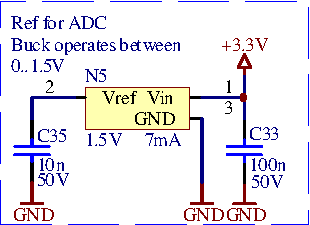
\includegraphics[width=.9\textwidth]{images/circuit/vref.pdf}
    \captionof{figure}{%
        \SI{1.5}{\volt} reference voltage for full-range operation of DACs
        and DACs
    }
    \label{fig:circuit:vref}
\end{minipage}



% **************************************************************************** %
\subsubsection{Enable and Under-Voltage Lockout circuit}
% **************************************************************************** %

The   LT3741's   \emph{Enable}   input   is   enabled   and   disabled   by  the
microcontroller's  $BUCK\_EN$ signal on one hand, on the other hand it is can be
forcibly  disabled  in  hardware  when  the  \SI{28}{\volt}  rail   drops  below
\SI{25}{\volt}. This  allows  for  a  controlled and predictable behavior of the
LT3741 during power-on  and power-off. The corresponding circuit can be found in
figure \ref{fig:circuit:uvlo}.

\begin{figure}[th!]
    \center
    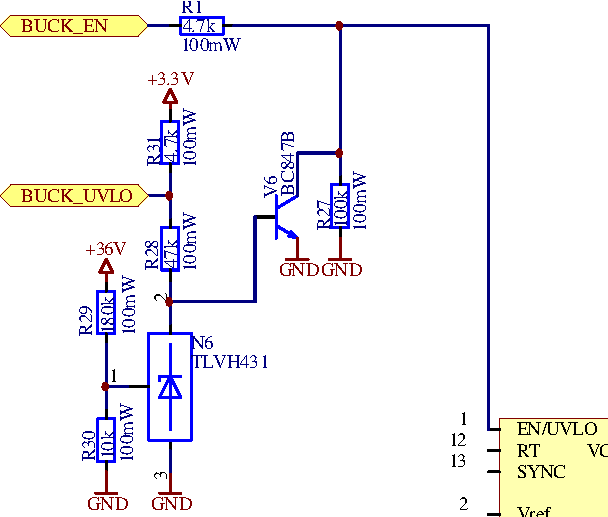
\includegraphics[width=.6\textwidth]{images/circuit/uvlo.pdf}
    \caption{Under-Voltage Lock-Out (UVLO) allows for controlled power-on and power-off of the controller}
    \label{fig:circuit:uvlo}
\end{figure}

In case of under-voltage, $N_6$ switches  on  and the transistor $V_6$ starts to
conduct,  thus  pulling  the  \emph{Enable}   input   to   \emph{Low}.   Voltage
$BUCK\_UVLO$ triggers an interrupt in the microcontroller.



